
% This LaTeX was auto-generated from MATLAB code.
% To make changes, update the MATLAB code and republish this document.

\documentclass[11pt]{article}
\usepackage[utf8]{inputenc}
\usepackage[T1]{fontenc}
\usepackage{amsthm}
\usepackage{enumitem}
\usepackage{amssymb}
\usepackage{amsmath}
\usepackage{amsfonts}
\usepackage[version=4]{mhchem}
\usepackage{stmaryrd}
\usepackage{mathrsfs}
\usepackage{bm}
\usepackage{graphicx}
\usepackage[export]{adjustbox}
\graphicspath{ {./images/} }
\usepackage{algorithm}
\usepackage{algorithmic}
\usepackage{makecell}  % 表格换行






 \usepackage{hyperref}
\hypersetup{
    colorlinks=true,     % 启用颜色链接
    linkcolor=blue,     % 内部链接的颜色
    citecolor=red,      % 引用文献的颜色
    urlcolor=blue,       % URL链接的颜色
    linktoc=red,      % 不影响目录链接颜色
}
\usepackage[a4paper, top=1in, bottom=1in, left=1in, right=1in]{geometry}

\title{
{\bf \huge Jacobi Polynomials}\\
{\bf \large Algorithms, Implementations, and Applications}
}
\author{Huaijin Wang}
\date{December 21, 2024}


\begin{document}


\newtheorem{definition}{Definition}[section]
\newtheorem{property}{Property}[section]
\newtheorem{lemma}{Lemma}[section]
\newtheorem{theorem}{Theorem}[]
\newtheorem{corollary}{Corollary}[section]
\newtheorem{remark}{Remark}[section]
\newtheorem{example}{Example}[]

\maketitle

\begingroup
\hypersetup{
    linkcolor=black,  % 将目录链接颜色设置为黑色
}
\tableofcontents
\endgroup


\newpage
\section{Introduction}
The \textit{Jacobi polynomials}, denoted by $J_n^{\alpha,\beta}(x)$, are orthogonal with respect to the \textit{Jacobi weight function} $\omega^{\alpha,\beta}(x):= (1-x)^\alpha (1+x)^\beta$ over $I:= (-1,1)$, namely,
\[
\int_{-1}^1 J_n^{\alpha, \beta}(x) J_m^{\alpha, \beta}(x) \omega^{\alpha, \beta}(x) d x=\gamma_n^{\alpha, \beta} \delta_{m n},
\]
where $\gamma_n^{\alpha, \beta}=\|J_n^{\alpha, \beta}\|_{\omega^{\alpha, \beta}}^2$. It is know that $J_n^{\alpha,\beta}$ is unique under the sense scaled by a constant (see \cite[Theorem 3.1]{shen2011}). And the $\gamma_n^{\alpha,\beta}$ is known as (see \cite[(3.109)]{shen2011})
\[
\gamma_n^{\alpha,\beta} =\frac{2^{\alpha+\beta+1} \Gamma(n+\alpha+1) \Gamma(n+\beta+1)}{(2 n+\alpha+\beta+1) n!\Gamma(n+\alpha+\beta+1)} .
\]

\section{Jacobi Polynomials}
For computing the values of $J_n^{\alpha,\beta}$ over any given $x\in[0,1]$, we leverage its three-term recurrence relation (see \cite[(3.110) and (3.111)]{shen2011}):
\begin{equation}
J_{n+1}^{\alpha, \beta}(x)=\left(a_n^{\alpha, \beta} x-b_n^{\alpha, \beta}\right) J_n^{\alpha, \beta}(x)-c_n^{\alpha, \beta} J_{n-1}^{\alpha, \beta}(x), n \geq 1,
\label{eq:rec}
\end{equation}
with the initial values:
\[
J_0^{\alpha, \beta}(x)=1, \quad J_1^{\alpha, \beta}(x)=\frac{1}{2}(\alpha+\beta+2) x+\frac{1}{2}(\alpha-\beta).
\]
Moreover, the coefficients are known:
\[
\begin{aligned}
a_n^{\alpha, \beta} & =\frac{(2 n+\alpha+\beta+1)(2 n+\alpha+\beta+2)}{2(n+1)(n+\alpha+\beta+1)}, \\
b_n^{\alpha, \beta} & =\frac{\left(\beta^2-\alpha^2\right)(2 n+\alpha+\beta+1)}{2(n+1)(n+\alpha+\beta+1)(2 n+\alpha+\beta)}, \\
c_n^{\alpha, \beta} & =\frac{(n+\alpha)(n+\beta)(2 n+\alpha+\beta+2)}{(n+1)(n+\alpha+\beta+1)(2 n+\alpha+\beta)} .
\end{aligned}
\]


\begin{algorithm}[htbp] 
    \caption{Computation of $J_n^{\alpha,\beta}(x)$.}
    \begin{algorithmic} \label{alg:japoly}
    	\REQUIRE{order $n$, $\alpha$, $\beta$ and $x$.}
        	 \STATE polylst = ones(size($x$)); polyn = polylst;
                \STATE poly = $0.5*(\alpha-\beta+(\alpha+\beta+2)*x$);
                \FOR{$k=2,\dots,n$}
                \STATE Compute $a^{\alpha,\beta}_{k-1}$, $b^{\alpha,\beta}_{k-1}$, and $c_{k-1}^{\alpha,\beta}$;                 
                \STATE polyn $\leftarrow (a_{k-1}^{\alpha,\beta} * x - b_{k-1}^{\alpha,\beta}) * \text{poly} - c_{k-1}^{\alpha,\beta} * \text{polylst}$;
                \STATE polylst $\leftarrow$ poly; poly $\leftarrow$ polyn; 
                \ENDFOR
                \RETURN{polyn.}
    \end{algorithmic}
\end{algorithm}

It can be observed from Algorithm \ref{alg:japoly} that the computation of $J_n^{\alpha,\beta}$ is easy and cheap. Due to the derivative relation (see \cite[(3.101)]{shen2011}):
\[
\partial_x^k J_n^{\alpha, \beta}(x)=d_{n, k}^{\alpha, \beta} J_{n-k}^{\alpha+k, \beta+k}(x), \quad n \geq k,
\]
where
\[
d_{n, k}^{\alpha, \beta}=\frac{\Gamma(n+k+\alpha+\beta+1)}{2^k \Gamma(n+\alpha+\beta+1)},
\]
it is straightforward to compute any derivatives of $J_n^{\alpha,\beta}$ via Algorithm \ref{alg:japoly}. And it is also straightforward to compute a string of $J_0^{\alpha,\beta},\cdots,J_n^{\alpha,\beta}$, with storing results at each step.

There are two \texttt{.m} files, \href{https://wanghuaijin.github.io/assets/codes/mFiles/japoly.m}{\texttt{japoly.m}} and \href{https://wanghuaijin.github.io/assets/codes/mFiles/japolym.m}{\texttt{japolym.m}}, to achieve the procedures. Both of them are developed by Wang Li-Lian on his website: \href{https://blogs.ntu.edu.sg/wanglilian/book/}{https://blogs.ntu.edu.sg/wanglilian/book/}. 



\begin{verbatim}
alp=0; bet=0; n=10; % n indicates the order of polynomials, n=0,1,...
x = linspace(-1,1,1000).';
[dy,y]=japoly(n,alp,bet,x);
subplot(1,2,1), plot(x,dy,'k'), grid on
axis([-1 1 -60.2 60.2]);
title('{$\partial_x J_{10}^{0,0}(x)$}','interpreter','LaTex','FontSize',14);
subplot(1,2,2), plot(x,y,'k'), grid on
axis([-1 1 -.75 1.15]);
title('{$J_{10}^{0,0}(x)$}','interpreter','LaTex','FontSize',14);
\end{verbatim}

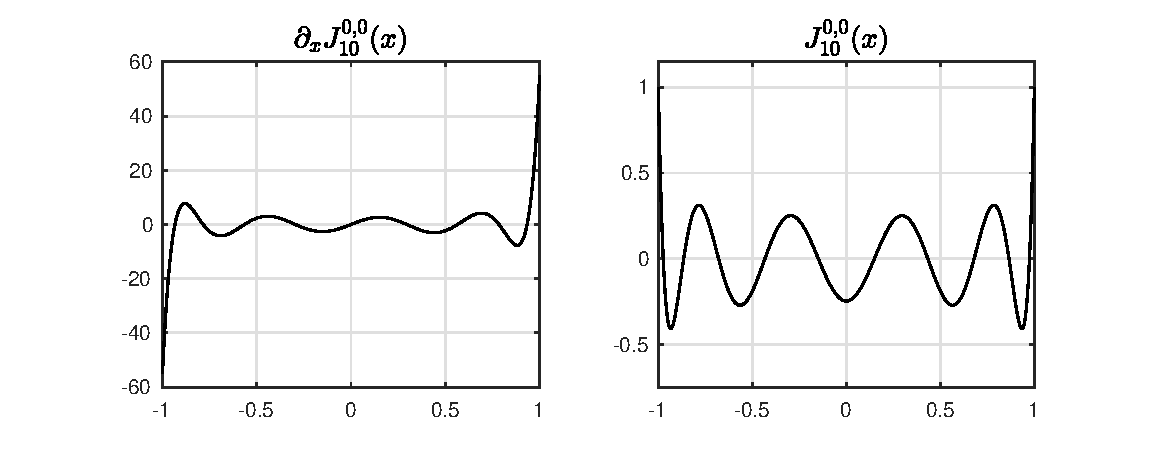
\includegraphics [scale=0.8]{eps1.eps}


\begin{verbatim}
alp=0; bet=0; n=10;
x = linspace(-1,1,1000).';
[DY,Y]=japolym(n,alp,bet,x);
% (k+1)-th row of DY (or Y) saves the value of J_k
% transform it to stack by colums
DY = DY.'; Y = Y.';
%
subplot(1,2,1), hold on, plot(x,DY(:,n+1),'k-','DisplayName', 'n=10'), 
plot(x,DY(:,n),'k--','DisplayName', 'n=9'), 
plot(x,DY(:,n-1),'k-.','DisplayName', 'n=8'), hold off
legend, grid on
axis([-1 1 -60.2 60.2]);
title(['{$\partial_x J_{n}^{0,0}(x)$}',' where n=10,9,8'],...
    'interpreter','LaTex','FontSize',14);
%
subplot(1,2,2), hold on, plot(x,Y(:,n+1),'k-','DisplayName', 'n=10'), 
plot(x,Y(:,n),'k--','DisplayName', 'n=9'), 
plot(x,Y(:,n-1),'k-.','DisplayName', 'n=8'), hold off
legend, grid on
axis([-1 1 -.75 1.15]);
title(['{$J_{n}^{0,0}(x)$}',' where n=10,9,8'],...
    'interpreter','LaTex','FontSize',14);
\end{verbatim}

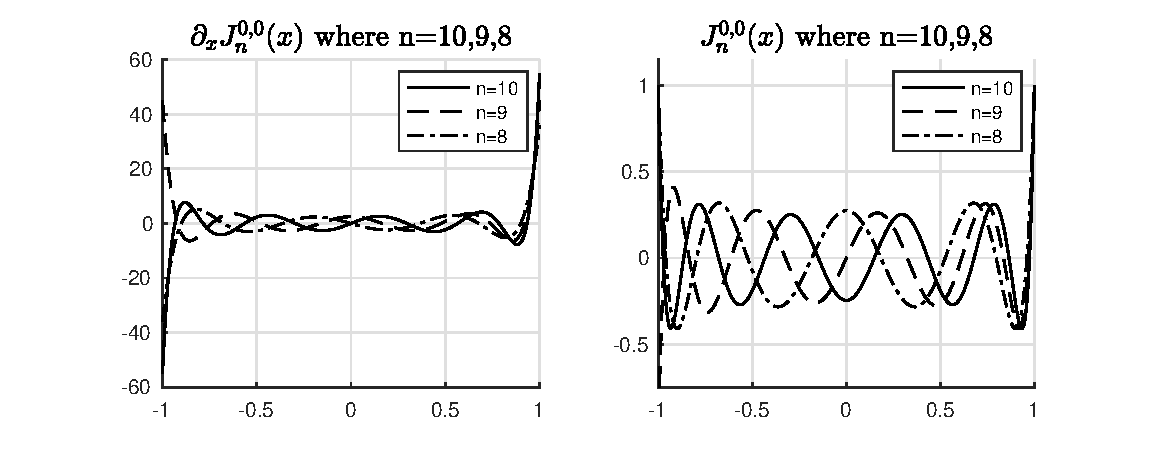
\includegraphics [scale=0.8]{eps2.eps}



\section{Jacobi Gauss-type Quadratures}

\subsection{Jacobi Gauss Quadrature}
Let $\{x_j\}_{j=0}^N$ be the zeros of $J_{N+1}^{\alpha,\beta}(x)$. It is known from \cite[Theorem 3.2]{shen2011} that $x_j$ are real, simple and lie in the interval $ (-1,1)$ for $j=0,\cdots,N$. The Lagrange basis polynomials associated with $\{x_j\}_{j=0}^N$ are given by
\[
h_j(x)=\prod_{i=0 ; i \neq j}^N \frac{x-x_i}{x_j-x_i}, \quad 0 \leq j \leq N.
\]
Let the \textit{weights}
\[
\omega_j=\int_a^b h_j(x) \omega(x) d x, \quad 0 \leq j \leq N.
\]
By \cite[Theorem 3.5]{shen2011}, we know that the nodes $\{x_j\}_{j=0}^N$ and weights $\{\omega_j\}_{j=0}^N$ are Gaussian. That is, the quadrature rule constituted by them satisfies
\[
\int_I p(x) \omega^{\alpha,\beta}(x) \mathrm{d} x = \sum_{j=0}^N p(x_j) \omega_j,\quad \forall p\in \mathbb{P}_{2N+1},
\]
where $\mathbb{P}_{2N+1}$ denotes the collection of polynomials with degree at most $2N+1$. Such quadrature rule are called Gauss quadrature. We know that all weights are positive. And Gauss quadrature shares highest \textit{algebraic accuracy}. In fact, there is no quadrature that have higher algebraic accuracy than Gauss quadrature.

Except for Chebyshev quadrature, other Jacobi quadratures have no closed form and numerical computation is required. A straight and simple way to this end is a method called \textit{eigenvalue method} due to \cite{golub1969}. Let 
\begin{equation}
A_{N+1}=\left[\begin{array}{ccccc}
a_0 & \sqrt{b_1} & & & \\
\sqrt{b_1} & a_1 & \sqrt{b_2} & & \\
& \ddots & \ddots & \ddots & \\
& & \sqrt{b_{N-1}} & a_{N-1} & \sqrt{b_N} \\
& & & \sqrt{b_N} & a_N
\end{array}\right],
\label{eq:jags-A}
\end{equation}
where $a_j$ and $b_j$ are determined by the coefficients of three-term recurrence relation \eqref{eq:rec}:
\[
\begin{aligned}
& a_j= \frac{b^{\alpha,\beta}_j}{a_j^{\alpha,\beta}} =\frac{\beta^2-\alpha^2}{(2 j+\alpha+\beta)(2 j+\alpha+\beta+2)}, \ 0\leqslant j\leqslant N\\
&b_j= \frac{1}{a^{\alpha,\beta}_{j-1}} \sqrt{\frac{a^{\alpha,\beta}_{j-1} c^{\alpha,\beta}_j}{a^{\alpha,\beta}_j}} =\frac{4 j(j+\alpha)(j+\beta)(j+\alpha+\beta)}{(2 j+\alpha+\beta-1)(2 j+\alpha+\beta)^2(2 j+\alpha+\beta+1)},\ 1\leqslant j\leqslant N .
\end{aligned}
\]
By \cite[Theorem 3.4 and Theorem 3.6]{shen2011}, we have
\begin{theorem}
Jacobi Gauss nodes $\{x_j\}_{j=0}^N$ are the eigenvalues of $A_{N+1}$. Let 
\[
\mathbf{Q}\left(x_j\right)=\left(Q_0\left(x_j\right), Q_1\left(x_j\right), \ldots, Q_N\left(x_j\right)\right)^T
\]
be the orthonormal eigenvector of $A_{N+1}$ corresponding to the eigenvalue $x_j$, i.e.,
\[
A_{N+1} \mathbf{Q}\left(x_j\right)=x_j \mathbf{Q}\left(x_j\right) \quad \text { with } \quad \mathbf{Q}\left(x_j\right)^T \mathbf{Q}\left(x_j\right)=1 .
\]
Then the Gaussian weights $\{\omega_j\}_{j=0}^N$ can be computed from the first component of the eigenvector $\mathbf{Q}(x_j)$ by using the formula:
\begin{equation}
\omega_j=\left[Q_0\left(x_j\right)\right]^2 \int_{-1}^1 \omega^{\alpha,\beta}(x) d x
= \left[Q_0\left(x_j\right)\right]^2 \frac{2^{\alpha+\beta+1} \Gamma(\alpha+1) \Gamma(\beta+1)}{(\alpha+\beta+1) \Gamma(\alpha+\beta+1)}, \quad 0 \leq j \leq N.
\label{eq:jags-ew}
\end{equation}
\end{theorem}

\begin{algorithm}[htbp] 
    \caption{Computation of Jacobi Gauss Quadrature.}
    \begin{algorithmic} \label{alg:jags}
    	\REQUIRE{ $N$, $\alpha$, and $\beta$.}
        	 \STATE Compute $A_{N+1}$ in \eqref{eq:jags-A};
                \STATE Determine the eigenpair $\{x_j, \mathbf{Q}(x_j)\}_{j=0}^N$ of $A_{N+1}$;
                \STATE Compute weights $\{\omega_j\}_{j=0}^N$ by \eqref{eq:jags-ew};
                \RETURN{$N+1$ Jacobi Gauss quadrature $\{x_j,\omega_j\}_{j=0}^N$.}
    \end{algorithmic}
\end{algorithm}

The eigenvalue method is based on the fact that Gaussian nodes correspond to the zeros of orthogonal polynomials, which satisfy a three-term recurrence relation. This approach for computing Gaussian nodes and weights is both classical and stable due to the well-structured nature of $A_{N+1}$. In most cases, this method is sufficiently accurate. However, its computational cost is 
 $O(N^2)$, and the results may be affected by the condition number of $A_{N+1}$. 
 
As a remedy, iterative methods, such as Newton's method, are often used with a good initial guess to compute Gaussian nodes, as they are more efficient and accurate. One possible initial guess is given in \cite[Theorem 8.9.1]{szego1975}. Alternatively, if computational cost is not a concern, the eigenvalues of  $A_{N+1}$ can be used as the initial guess to achieve higher accuracy. Once the Gaussian nodes $\{x_j\}_{j=0}^N$ are computed, the Gaussian weights can be determined in following formula (see \cite[(3.131)]{shen2011}):
\begin{equation}
\omega_j =\frac{\widetilde{G}_N^{\alpha, \beta}}{\left(1-x_j^2\right)\left[\partial_x J_{N+1}^{\alpha, \beta}\left(x_j\right)\right]^2}, \ 0\leqslant j \leqslant N,
\label{eq:jags-w}
\end{equation}
where
\[
\widetilde{G}_N^{\alpha, \beta}=\frac{2^{\alpha+\beta+1} \Gamma(N+\alpha+2) \Gamma(N+\beta+2)}{(N+1)!\Gamma(N+\alpha+\beta+2)}.
\]
It is evident that with a good initial guess, computing Gaussian nodes and then determining Gaussian weights using \eqref{eq:jags-w} may require only $O(N)$ computational cost.

There is a \texttt{.m} file, \href{https://wanghuaijin.github.io/assets/codes/mFiles/jags.m}{\texttt{jags.m}}, to compute Jacobi Gauss quadrature, which is developed by Wang Li-Lian on his website: \href{https://blogs.ntu.edu.sg/wanglilian/book/}{https://blogs.ntu.edu.sg/wanglilian/book/}. \texttt{jags.m} computes the Gaussian nodes by the eigenvalues of $A_{N+1}$, and determine the Gaussian weights via \eqref{eq:jags-w}. It is easy to execute the \texttt{jags.m} command as follows:
\begin{verbatim}
n = 15; alp=1/2; bet=0;
[x,w]=jags(n,alp,bet);
% returns n nodes Gauss quadrature
\end{verbatim}

\subsection{Jacobi Gauss-Radau Quadrature}
Jacobi Gauss-Radau quadrature is a special type of Gauss quadrature with one of its nodes is fixed on the boundary. That is, $\{x_j,\omega_j\}_{j=0}^N$ with $x_0 = -1$ (or $x_N=1$) satisfy
\[
\int_I p(x) \omega^{\alpha,\beta}(x) \mathrm{d} x = \sum_{j=0}^N p(x_j) \omega_j,\quad \forall p \in \mathbb{P}_{2N}.
\]

\begin{theorem}[Theorem 3.26, \cite{shen2011}]
Let $x_0 = -1$ and $\{x_j\}_{j=1}^N$ be the zeros of $J_{N}^{\alpha,\beta+1}(x)$, and
\begin{equation}
\omega_0=\frac{2^{\alpha+\beta+1}(\beta+1) \Gamma^2(\beta+1) N!\Gamma(N+\alpha+1)}{\Gamma(N+\beta+2) \Gamma(N+\alpha+\beta+2)},
\label{eq:jagsrd1-w}
\end{equation}
\[
\omega_j =\frac{1}{\left(1-x_j\right)\left(1+x_j\right)^2} \frac{\widetilde{G}_{N-1}^{\alpha, \beta+1}}{\left[\partial_x J_N^{\alpha, \beta+1}\left(x_j\right)\right]^2}, \quad 1 \leq j \leq N .
\]
where
\[
\widetilde{G}_{N-1}^{\alpha, \beta+1}=\frac{2^{\alpha+\beta+2} \Gamma(N+\alpha+1) \Gamma(N+\beta+2)}{N! \Gamma(N+\alpha+\beta+2)}.
\]
Then $\{x_j,\omega_j\}_{j=0}^N$ is the desired Jacobi Gauss-Radau quadrature with $x_0=-1$ fixed.
\end{theorem}

Similarly, we can show that
\begin{theorem}
Let $x_N = 1$ and $\{x_j\}_{j=0}^{N-1}$ be the zeros of $J_{N}^{\alpha+1,\beta}(x)$, and
\begin{equation}
\omega_N=\frac{2^{\alpha+\beta+1}(\alpha+1) \Gamma^2(\alpha+1) N!\Gamma(N+\beta+1)}{\Gamma(N+\alpha+2) \Gamma(N+\alpha+\beta+2)},
\label{eq:jagsrd2-w}
\end{equation}
\[
\omega_j =\frac{1}{\left(1-x_j\right)^2\left(1+x_j\right)} \frac{\widetilde{G}_{N-1}^{\alpha+1, \beta}}{\left[\partial_x J_N^{\alpha+1, \beta}\left(x_j\right)\right]^2}, \quad 0 \leq j \leq N-1 .
\]
where
\[
\widetilde{G}_{N-1}^{\alpha+1, \beta}=\frac{2^{\alpha+\beta+2} \Gamma(N+\beta+1) \Gamma(N+\alpha+2)}{N! \Gamma(N+\alpha+\beta+2)}.
\]
Then $\{x_j,\omega_j\}_{j=0}^N$ is the desired Jacobi Gauss-Radau quadrature with $x_N=1$ fixed.
\end{theorem}

We denote $\{\xi_{G,N,j}^{\alpha,\beta}, \omega_{G,N,j}^{\alpha,\beta} \}_{j=0}^N$ as the $N$ nodes Gauss quadrature with respect to weight function $\omega^{\alpha,\beta}(x)$, and $\{\xi_{R_l,N,j}^{\alpha,\beta}, \omega_{R_l,N,j}^{\alpha,\beta} \}_{j=0}^N$ the Gauss-Radau quadrature with $\xi_{R_l,N,0}^{\alpha,\beta} = -1$ fixed. Then by \cite[(3.140)]{shen2011} we have 
\begin{equation}
\xi_{R_l, N, j}^{\alpha, \beta}=\xi_{G, N-1, j-1}^{\alpha, \beta+1}, \quad \omega_{R_l, N, j}^{\alpha, \beta}=\frac{\omega_{G, N-1, j-1}^{\alpha, \beta+1}}{1+\xi_{G, N-1, j-1}^{\alpha, \beta+1}}, \quad 1 \leq j \leq N.
\label{eq:jagsrd1-gs}
\end{equation}
Similarly, we denote $\{\xi_{R_r,N,j}^{\alpha,\beta}, \omega_{R_r,N,j}^{\alpha,\beta} \}_{j=0}^N$ as the Gauss-Radau quadrature with $\xi_{R_r,N,N}^{\alpha,\beta}=1$ fixed. Then
\begin{equation}
\xi_{R_r, N, j}^{\alpha, \beta}=\xi_{G, N-1, j}^{\alpha+1, \beta}, \quad \omega_{R_r, N, j}^{\alpha, \beta}=\frac{\omega_{G, N-1, j}^{\alpha+1, \beta}}{1-\xi_{G, N-1, j}^{\alpha+1, \beta}}, \quad 0 \leq j \leq N-1.
\label{eq:jagsrd2-gs}
\end{equation}
Both \eqref{eq:jagsrd1-gs} and \eqref{eq:jagsrd2-gs} inform us that the computation of Jacobi Gauss-Radau quadratures can be transformed into computing Jacobi Gauss quadratures.

\begin{algorithm}[htbp] 
    \caption{Computation of Jacobi Gauss-Radau Quadrature with $x_0=-1$ fixed.}
    \begin{algorithmic} \label{alg:jagsrd1}
    	\REQUIRE{ $N$, $\alpha$, and $\beta$.}
        	 \STATE Compute Jacobi Gauss quadrature $\{x_j,\omega_j\}_{j=1}^N$ via Algorithm \ref{alg:jags} with $N-1$, $\alpha$ and $\beta+1$;
                \STATE Let $x_0=-1$, and determine $\omega_0$ by \eqref{eq:jagsrd1-w};
                \STATE Compute weights $\omega_j \leftarrow \omega_j/(1+x_j)$ for $j=1,\cdots,N$;
                \RETURN{$N+1$ Jacobi Gauss-Radau quadrature $\{x_j,\omega_j\}_{j=0}^N$.}
    \end{algorithmic}
\end{algorithm}


\begin{algorithm}[htbp] 
    \caption{Computation of Jacobi Gauss-Radau Quadrature with $x_N= 1$ fixed.}
    \begin{algorithmic} \label{alg:jagsrd2}
    	\REQUIRE{ $N$, $\alpha$, and $\beta$.}
        	 \STATE Compute Jacobi Gauss quadrature $\{x_j,\omega_j\}_{j=0}^{N-1}$ via Algorithm \ref{alg:jags} with $N-1$, $\alpha+1$ and $\beta$;
                \STATE Let $x_N=1$, and determine $\omega_N$ by \eqref{eq:jagsrd2-w};
                \STATE Compute weights $\omega_j \leftarrow \omega_j/(1-x_j)$ for $j=0,\cdots,N-1$;
                \RETURN{$N+1$ Jacobi Gauss-Radau quadrature $\{x_j,\omega_j\}_{j=0}^N$.}
    \end{algorithmic}
\end{algorithm}

There are two \texttt{.m} files, \href{https://wanghuaijin.github.io/assets/codes/mFiles/jagsrd1.m}{\texttt{jagsrd1.m}} and \href{https://wanghuaijin.github.io/assets/codes/mFiles/jagsrd2.m}{\texttt{jagsrd2.m}}, to compute Jacobi Gauss-Radau quadratures. \texttt{jagsrd1.m} computes the Gauss-Radau quadrature with left-end point fixed, while \texttt{jagsrd2.m} treats the other case. It is easy to execute the commands as follows:
\begin{verbatim}
n = 15; alp=1/2; bet=0;
[x,w]=jagsrd1(n,alp,bet); % returns n nodes Gauss-Radau quadrature with x0=-1 
[x,w]=jagsrd2(n,alp,bet); % returns n nodes Gauss-Radau quadrature with xN=1 
\end{verbatim}


\subsection{Jacobi Gauss-Lobatto Quadrature}
Jacobi Gauss-Lobatto quadrature is a special type of Guass quadrature with two of its nodes are fixed on the boundary. That is $\{x_j,\omega_j\}_{j=0}^N$ with $x_0=-1$ and $x_N=1$ satisfy
\[
\int_I p(x) \omega(x) \mathrm{d} x = \sum_{j=0}^N p(x_j) \omega_j,\quad \forall p\in \mathbb{P}_{2N-1}.
\]

\begin{theorem}[Theorem 3.27 in \cite{shen2011}]
 Let $x_0 = -1$, $x_N = 1$ and $\{x_j\}_{j=1}^{N-1}$ be the zeros of $J_{N-1}^{\alpha+1,\beta+1}(x)$, and let
 \begin{equation}
 \begin{aligned}
\omega_0 & =\frac{2^{\alpha+\beta+1}(\beta+1) \Gamma^2(\beta+1) \Gamma(N) \Gamma(N+\alpha+1)}{\Gamma(N+\beta+1) \Gamma(N+\alpha+\beta+2)}, \\
\omega_N & =\frac{2^{\alpha+\beta+1}(\alpha+1) \Gamma^2(\alpha+1) \Gamma(N) \Gamma(N+\beta+1)}{\Gamma(N+\alpha+1) \Gamma(N+\alpha+\beta+2)}, \\
\omega_j &  =\frac{1}{\left(1-x_j^2\right)^2} \frac{\widetilde{G}_{N-2}^{\alpha+1, \beta+1}}{\left[\partial_x J_{N-1}^{\alpha+1, \beta+1}\left(x_j\right)\right]^2}, \quad 1 \leq j \leq N-1,
\end{aligned}
\label{eq:jagslb-w}
 \end{equation}
 where
\[
\widetilde{G}_{N-2}^{\alpha+1, \beta+1}=\frac{2^{\alpha+\beta+3} \Gamma(N+\alpha+1) \Gamma(N+\beta+1)}{(N-1)! \Gamma(N+\alpha+\beta+2)}.
\]
Then $\{x_j,\omega_j\}_{j=0}^N$ is the desired Jacobi Gauss-Lobatto quadrature with $x_0=-1$ and $x_N=1$ fixed.
\end{theorem}
We denote $\{\xi_{G,N,j}^{\alpha,\beta}, \omega_{G,N,j}^{\alpha,\beta} \}_{j=0}^N$ as the $N$ nodes Gauss quadrature with respect to weight function $\omega^{\alpha,\beta}(x)$, and $\{\xi_{L,N,j}^{\alpha,\beta}, \omega_{L,N,j}^{\alpha,\beta} \}_{j=0}^N$ the Gauss-Lobatto quadrature with $\xi_{L,N,0}^{\alpha,\beta} = -1$ and $\xi_{L,N,N}^{\alpha,\beta} = 1$ fixed. Then by \cite[(3.141)]{shen2011} we have
\begin{equation}
\xi_{L, N, j}^{\alpha, \beta}=\xi_{G, N-2, j-1}^{\alpha+1, \beta+1}, \quad \omega_{L, N, j}^{\alpha, \beta}=\frac{\omega_{G, N-2, j-1}^{\alpha+1, \beta+1}}{1-\left(\xi_{G, N-2, j-1}^{\alpha+1, \beta+1}\right)^2}, \quad 1 \leq j \leq N-1.
\label{eq:jagslb-gs}
\end{equation}

\eqref{eq:jagslb-gs} informs us that the computation of Jacobi Gauss-Lobatto quadrature can be implemented via Jacobi Gauss quadrature.
% 
\begin{algorithm}[htbp] 
    \caption{Computation of Jacobi Gauss-Lobatto Quadrature.}
    \begin{algorithmic} \label{alg:jagslb}
    	\REQUIRE{ $N$, $\alpha$, and $\beta$.}
        	 \STATE Compute Jacobi Gauss quadrature $\{x_j,\omega_j\}_{j=1}^{N-1}$ via Algorithm \ref{alg:jags} with $N-2$, $\alpha+1$ and $\beta+1$;
                \STATE Let $x_0=-1$ and $x_N=1$, and determine $\omega_0$ and $\omega_N$ by \eqref{eq:jagslb-w};
                \STATE Compute weights $\omega_j \leftarrow \omega_j/(1-x_j^2)$ for $j=1,\cdots,N-1$;
                \RETURN{$N+1$ Jacobi Gauss-Lobatto quadrature $\{x_j,\omega_j\}_{j=0}^N$.}
    \end{algorithmic}
\end{algorithm}

There is a \texttt{.m} file, \href{https://wanghuaijin.github.io/assets/codes/mFiles/jagslb.m}{\texttt{jagslb.m}}, to compute Jacobi Gauss-Lobatto quadrature, which is developed by Wang Li-Lian on his website: \href{https://blogs.ntu.edu.sg/wanglilian/book/}{https://blogs.ntu.edu.sg/wanglilian/book/}.
It is easy to execute the commands as follows:
\begin{verbatim}
n = 15; alp=1/2; bet=0;
[x,w]=jagslb(n,alp,bet); % returns n nodes Gauss-Lobatto quadrature
\end{verbatim}

\section{Jacobi Spectral Method}
\section{Reproduction: \cite{hou2019}}




\newpage
\begin{thebibliography}{99}
\bibitem[Shen (2011)]{shen2011} \href{https://wanghuaijin.github.io/assets/ref/books/Shen2011.pdf}{Shen J, Tang T, Wang L L. Spectral methods: algorithms, analysis and applications[M]. Springer Science \& Business Media, 2011.}
\bibitem[Golub (1969)]{golub1969} \href{https://wanghuaijin.github.io/assets/ref/articles/Golub1969.pdf}{Golub G H, Welsch J H. Calculation of Gauss quadrature rules[J]. Mathematics of computation, 1969, 23(106): 221-230.}
\bibitem[Szego (1975)]{szego1975} \href{https://wanghuaijin.github.io/assets/ref/books/Szego1975.pdf}{Szego G. Orthogonal polynomials[M]. American Mathematical Soc., 1975.}
\bibitem[Hou (2019)]{hou2019} Hou D, Lin Y, Azaiez M, et al. A Müntz-collocation spectral method for weakly singular Volterra integral equations[J]. Journal of scientific computing, 2019, 81(3): 2162-2187.

\end{thebibliography}


\end{document}

